\section{GPU}
\label{sec:cuda}

The development of a GPU implementation of \polu was divided into two phases.
The initial implementation consisted only on getting a working implementation, with basic, somewhat naive kernels implemented to move \computeflux and \update computations to the GPU.
After a comparison with the other implementation done at that point, it was decided to invest more time in the CUDA version.
Not only was its execution time much better than other implementations, since it was still a naive implementation it was most likely to still have room for improvements.

\subsection{Load Balance}
\label{subsec:cuda:load}

The nature of the algorithm allows for an easy and effective load balancing strategy. In CPU implementations, \computeflux iterates over all edges, and \update over all cells, and the workload of each iteration is homogeneous and free of dependencies, as already shown in \cref{subsec:omp:load}. So the balancing strategy can consist, for both kernels, in simply assigning one iteration to one CUDA thread. In \computeflux, one CUDA thread will be responsible for computing the flux for a specific edge, while in \update, one CUDA thread will update the pollution of a specific cell.

In order to use the ideal block size was for each kernel, CUDA Occupancy Calculator \cite{cuda_documentation} was used, having in consideration the CUDA Capability of the device used (see \cref{sec:env}) and the amount of registers and memory used by each kernel, which is accessible via nvcc. Using the block size recommended by the CUDA Occupancy Calculator does not guarantee better performance, and may actually result in unwanted behavior, such as register spilling, or greater branch divergente, experiments were made with different block sizes to detect which provided better results.

\subsection{Optimizations}
\label{subsec:cuda:load}

One of the first optimizations done comes from a simplification already explained in \todo[inline]{Onde é que explicas que a reduction pode ser feita fora do loop?}. The initial implementation, like the CPU versions, relied on a reduction to compute the maximum velocity after each iteration. The reduction used was based on the most optimized implementation provided in the NVidia samples, and is, according to the author, one of the most optimized CUDA reductions.

But the simplification of moving the maximum velocity computation to outside of the loop didn't rely only on the reduction, as that was only the final step of the computation. There was also added workload to the \computeflux kernel, which had to compute the velocity in each CUDA thread. More than the amount of operations, this had a considerable impact on the amount of registers used by the kernel, and it was noted that after its removal, there was also some improvements in \computeflux, and consequentely, in the main loop. This can be seen in \cref{fig:time_computeflux}.

\subsubsection{Second Phase}
\label{subsubsec:cuda:load:second}

On the second phase of the development of a CUDA implementation, more attention was given to the individual performance of the kernels. A lot of experiments were done with different kernel implementations, in order to test different approaches to eliminate memory accesses, and reduce or eliminate divergent branches.

While this provided small improvements to kernel execution time, consequentely decreasing the main loop time considerably, the better speedup was achieved after a division operation was removed from the \update, which computed a ratio between the length of an edge and the area of a cell. This was achieved by precomputing a matrix with the value of the ratio prior to the main loop. This required a considerable  amount of additional memory to be used on the GPU, but since the problem is not bound by total size (biggest test case used consisted of less than 100MB) and division operations are very costly to a GPU, this showed large improvements for the \update kernel, as shown in \cref{fig:time_update}

\begin{figure}[!htp]
	\begin{subfigure}[b]{\columnwidth}
		\centering
		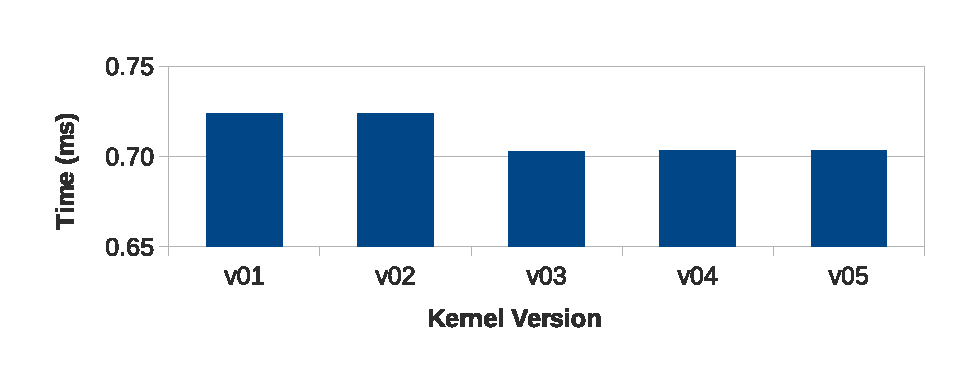
\includegraphics[width=\columnwidth]{graph_compute_flux}
		\caption{\computeflux}
		\label{fig:time_computeflux}
	\end{subfigure}
	\begin{subfigure}[b]{\columnwidth}
		\centering
		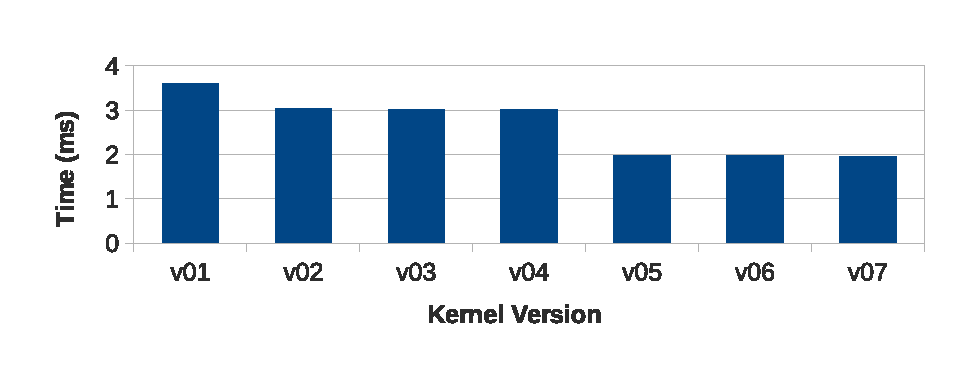
\includegraphics[width=\columnwidth]{graph_update}
		\caption{\update}
		\label{fig:time_update}
	\end{subfigure}

	\caption{Indivudual kernel speedups. Times are the average for a single kernel call}
	\label{fig:time_kernles}
\end{figure}

Times shown in \cref{fig:time_kernels} were measured using the CUDA Events API, which allows measurements of GPU events, excluding the callback overhead of issuing a kernel call. That, along with the fact that both kernels have considerably short and simple code, explains the low times, even for the initial versions. Even so, the removal of the division operation, along with other smaller tweaks, allowed the execution time of the \update kernel to be almost halved.

Since CUDA Events API only measures events with a precision of 0.5 ms \cite{cuda_library_documentation}, and the execution time is small, no immediate changes can be seen between some of the versions. However, since later kernels are the result of aggregating most optimizations from previous versions, intermediate results are still shown.

\subsection{Mesh ordering impact}
\todo[inline,color=green!40]{Explain how better ordering of cells/edges should, theoretically, be useful to increase coalesced memory accesses}
\todo[inline,color=green!40]{Talk about the simple optimization attempt (mesh reorder) and its poor (maybe null?) impact on performance}

\subsection{Results}
\label{subsec:cuda:results}

\todorev{Last revised on Sun, July 1 at 00:27 by pfac}

Results for the CUDA implementations are here presented in the form of speedups, relatively to the original raw version of \polu (see \cref{sec:env,sec:method} for details on the environmental setup and methodology used, respectively).
Results were measured by comparing both the first, more naive CUDA implementation, and the last implementation, with better kernels and the divison removed from \update kernel.
Some intermediate implementations were also created, since optimizations were agregated by each new kernel version created, but only the final results of the optimizations are shown in \cref{fig:cuda:results}.

\begin{figure}[!htp]
	\centering
	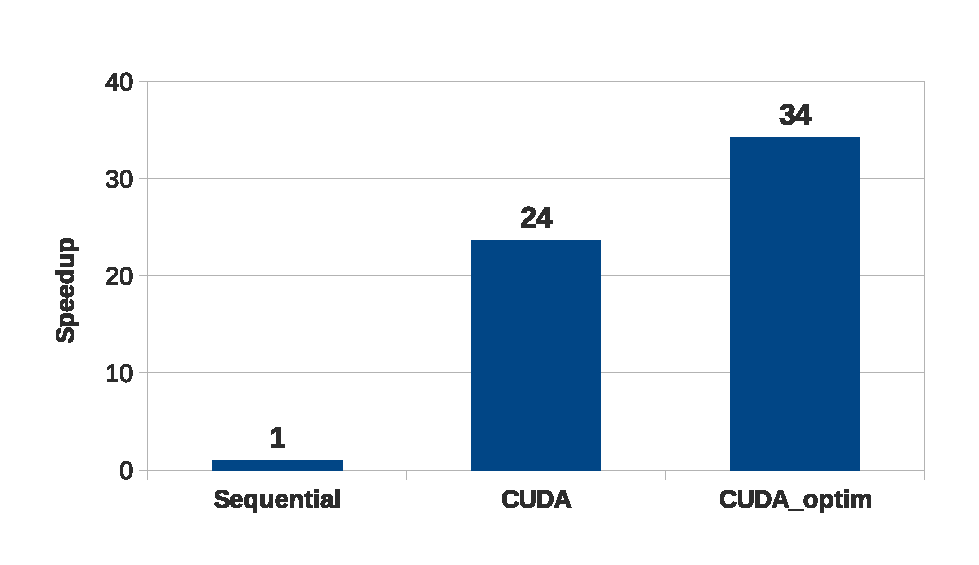
\includegraphics[width=\columnwidth]{graph_comparison_cuda}
	\caption{CUDA implementation speedups}
	\label{fig:cuda:results}
\end{figure}

The initial CUDA version already showed significant performance gains, almost matching the best speedup achieved with the OpenMP implementation in \cref{sec:omp}.
Optimizations were able to boost this speedup even further, achieving a total speedup of 34, the best one in this project.

However, the gain against the OpenMP version is not as large as previously expected, since this problem seemed extremelly well suited to a massively parallel approach, like the one employed by CUDA.
This is a result of the limited test case size, which was generated using a conversion utility provided with \polu, that converts \texttt{gmsh} output to a XML file readable by \polu.
This utility was not subject to optimizations or parallelization, but uses an algorithm in the order of $\Theta(N^3)$, making the generation of larger test cases impossible due to time limitations.
The test cases available, which only go up to 62MB, still do not reach the maximum capacity of the GPU, which may benefit from the addition of even more threads.

Given the chance to test this theory, this could show much greater scalability for the CUDA implementation.

